\iffalse
\documentclass[12pt]{article}
\usepackage{graphicx}
\usepackage[none]{hyphenat}
\usepackage{graphicx}
\usepackage{listings}
\usepackage[english]{babel}
\usepackage{graphicx}
\usepackage{caption} 
\usepackage{booktabs}
\usepackage{array}
\usepackage{amssymb} % for \because
\usepackage{amsmath}   % for having text in math mode
\usepackage{extarrows} % for Row operations arrows
\usepackage{listings}
\usepackage[utf8]{inputenc}
\lstset{
  frame=single,
  breaklines=true
}
\usepackage{hyperref}
  
%Following 2 lines were added to remove the blank page at the beginning
\usepackage{atbegshi}% http://ctan.org/pkg/atbegshi
\AtBeginDocument{\AtBeginShipoutNext{\AtBeginShipoutDiscard}}


%New macro definitions
\newcommand{\mydet}[1]{\ensuremath{\begin{vmatrix}#1\end{vmatrix}}}
\providecommand{\brak}[1]{\ensuremath{\left(#1\right)}}
\newcommand{\solution}{\noindent \textbf{Solution: }}
\newcommand{\myvec}[1]{\ensuremath{\begin{pmatrix}#1\end{pmatrix}}}
\providecommand{\norm}[1]{\left\lVert#1\right\rVert}
\providecommand{\abs}[1]{\left\vert#1\right\vert}
\let\vec\mathbf

\begin{document}

\begin{center}
\title{\textbf{VECTORS}}
\date{\vspace{-5ex}} %Not to print date automatically
\maketitle
\end{center}

\section{10$^{th}$ Maths - EXERCISE-7.2}

\begin{enumerate}
\item Find the coordinates of the points of trisection of the line segment joining $\vec(4 ,-1) \text{ and } \vec(-2,-3)$ 
\end{enumerate}
\fi
Let the given points be
\begin{align}
\vec{Q}=\myvec{4\\ -1} ,
\vec{P}=\myvec{-2\\ -3}
\end{align}
Using section formula
\begin{align}
\vec{R}&=\frac{\vec{Q}+n\vec{P}}{1+n}
\end{align}
Choosing $n = \frac{1}{2}$,
\begin{align}
\vec{R}&=\frac{1}{1+\frac{1}{2}}\brak{\myvec{4\\-1}+\frac{1}{2}\myvec{-2\\-3}}\\
&=\myvec{2\\ \frac{-5}{3}}\\
\end{align}
and choosing $n = 2$
\begin{align}
\vec{S}&=\frac{1}{1+\frac{2}{1}}\brak{\myvec{4\\-1}+\frac{2}{1}\myvec{-2\\-3}}\\
&=\myvec{0\\ \frac{-7}{3}}
\end{align}
which are the desired points of trisection.  These are plotted in Fig. 
		\ref{fig:chapters/10/7/2/2/Figure}
\begin{figure}[h]
\centering
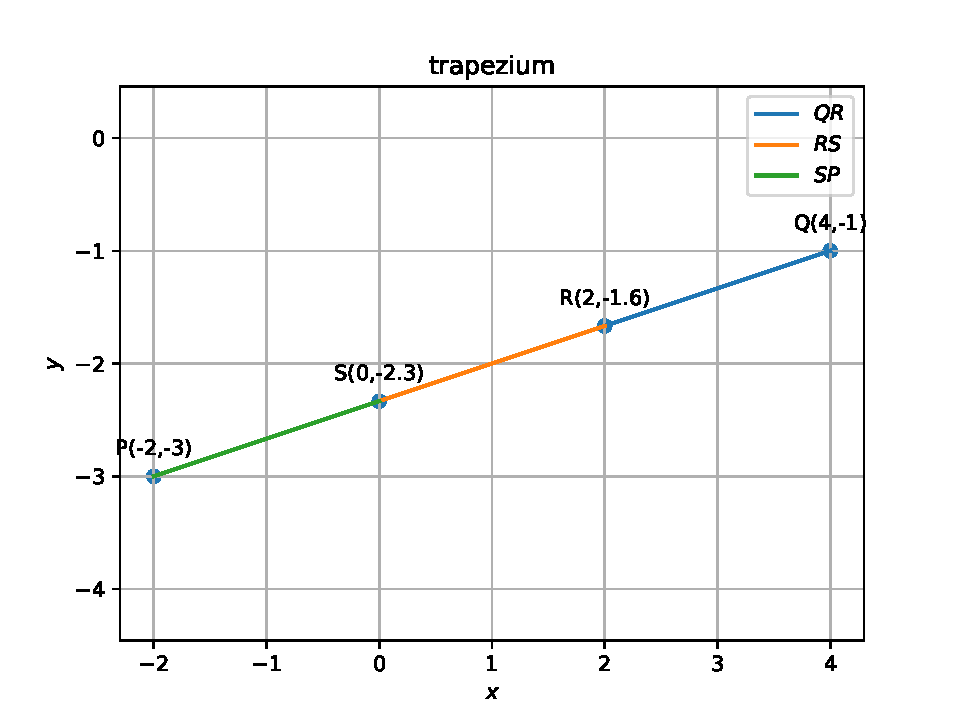
\includegraphics[width=\columnwidth]{chapters/10/7/2/2/figs/dj.pdf}
\caption{}
		\label{fig:chapters/10/7/2/2/Figure}
\end{figure}
